\chapter{Variance-Bias Trade-off}
L'errore di generalizzazione è determinato da diversi fattori:
\begin{itemize}
  \item \textbf{Irreducible Error}: errore che dipende dalla qualità e dalla quantità dei dati che non può essere ridotto.
  \item \textbf{Variance}: errore dovuto alla sensibilità del modello alle piccole variazioni nei dati.
        Un alta varianza determina un elevato adattamento ai dati.
  \item \textbf{Bias}: errore che misura quanto le predizioni del modello si distaccano dai valori attesi.
        Un alto bias determina una bassa accuratezza.
\end{itemize}

\begin{figure}[ht]
  \centering
  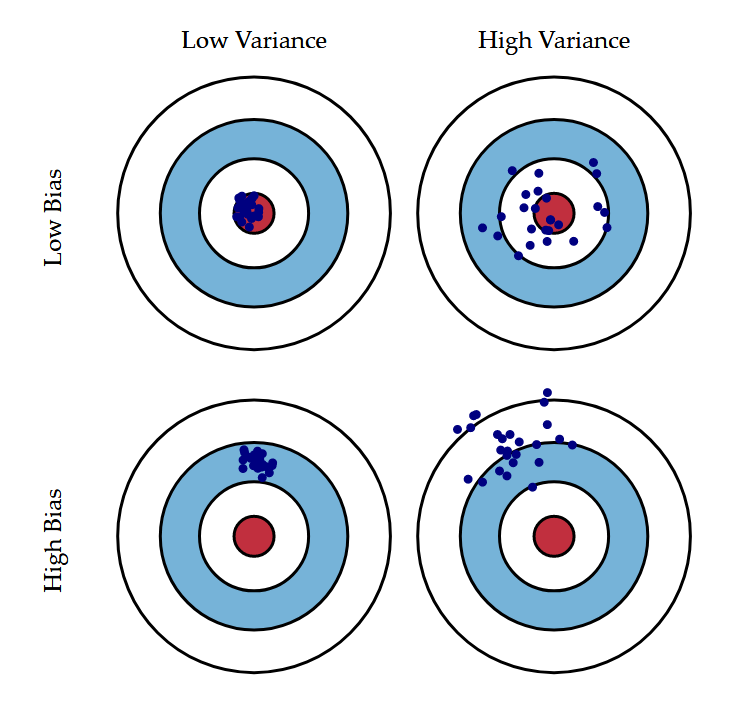
\includegraphics[width=0.5\linewidth]{images/bias-variance.png}
  \caption{Illustrazione grafica di bias e variance \cite{img:bias-variance}.}
\end{figure}

Un modello con bias alto fa delle assunzioni troppo semplici sui dati (underfitting).
Mentre un modello con alta variance si adatta troppo ai dati (overfitting).
Un buon modello deve avere bassa varianza e basso bias.

La complessità del modello influenza bias e variance. All'aumentare della complessità la variance crescerà e il bias decrescerà.

\begin{figure}[ht]
  \centering
  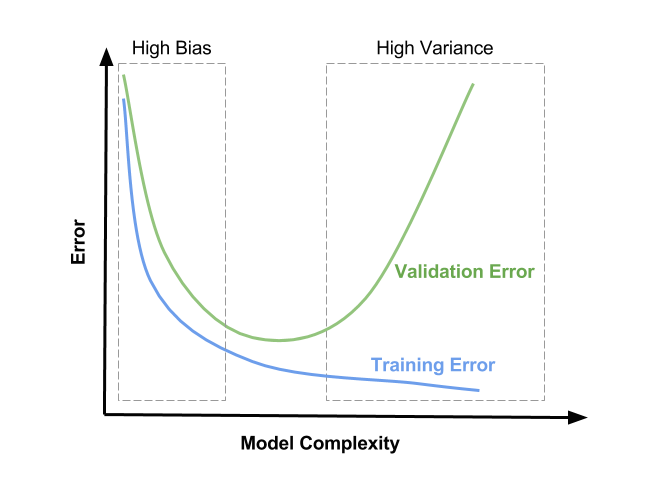
\includegraphics[width=0.6\linewidth]{images/Bias-Variance-Tradeoff-In-Machine-Learning-1.png}
  \caption{Bias-variance tradeoff \cite{img:model-complexity}.}
\end{figure}

Confrontando l'errore sul train set e sul validation set è possibile osservare il comportamento di bias e variance.

Quando le due curve di errore sono vicine significa che la varianza è bassa e si adatta ai dati di entrambi gli insiemi.
Viceversa quando le curve sono distanti la varianza è alta e si adatta molto sul train set (overfitting).

Se l'errore è alto vuol dire che il bias è alto e che il modello è troppo semplice e non riesce a rappresentare i dati (underfitting).

\begin{figure}[ht]
  \centering
  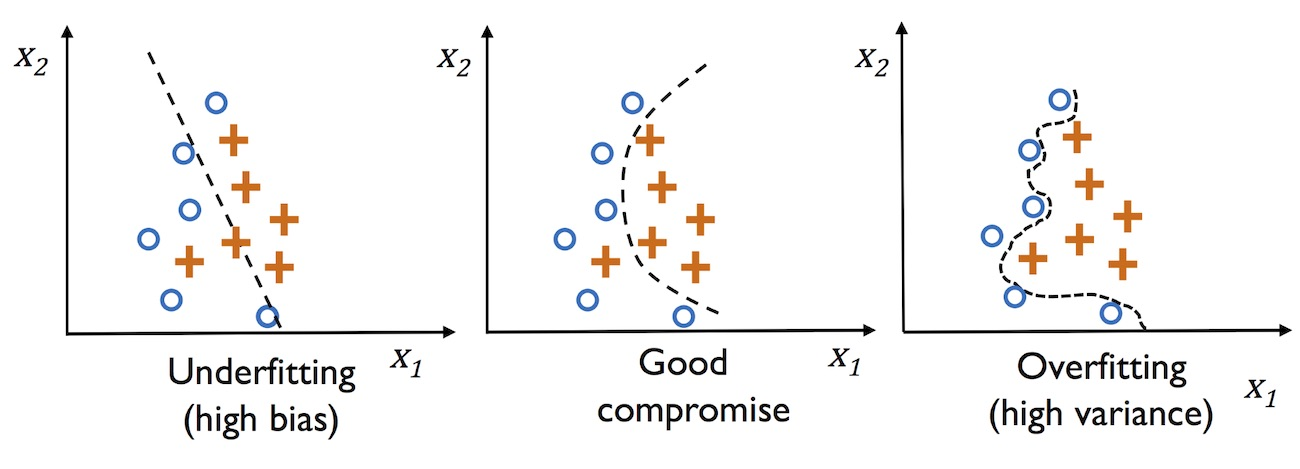
\includegraphics[width=0.9\linewidth]{images/fitting.jpeg}
  \caption{Underfitting e overfitting \cite{RaschkaMirjalili2019}.}
\end{figure}

Per ridurre l'errore di generalizzazione (variance e bias) è possibile usare tecniche di regolarizzazione, boosting o bagging.
